\documentclass[a4paper,14pt]{extarticle}
\usepackage[utf8]{inputenc}
\usepackage[T1]{fontenc}
\usepackage[russian]{babel}
\usepackage{indentfirst}
\usepackage{geometry}
\usepackage{fontspec}
\usepackage{wrapfig}
\usepackage[explicit]{titlesec}
\usepackage{longtable}
\usepackage{graphicx}
\usepackage{float}

\geometry{
    left=30mm,
    top=20mm,
    bottom=20mm,
    right=15mm,
}

\setmainfont{Times New Roman}

\titleformat{\section}
{\normalfont}{\bfseries \thesection.}{4pt}{\bfseries #1}

\titleformat{\subsection}
{\normalfont}{\bfseries \thesubsection.}{4pt}{\bfseries #1}

\begin{document}

\section{Цели}

Целью данной лабораторной работы является разработка архитектуры базы данных для интернет-площадки по продаже креативных вещей.

\section{Задачи}

Для достижения поставленных целей необходимо решить следующие задачи:
\begin{itemize}
    \item анализ предметной области;
    \item анализ существующих аналогов;
    \item выделение основных сущностей;
    \item определение связей между сущностями;
    \item создание UML-модели.
\end{itemize}

\section{Необходимость}

<<Креатистор>> -- это интернет-площадка для креативных людей, интересных идей и уникальных товаров.

На рынке существует множество различных магазинов креативных товаров. Однако мы готовы предложить совершенно новый уровень сервиса. Мы не покупаем и не продаем товары, мы предоставляем площадку, на которой могут встретится продавцы и покупатели. Мы ориентированы не масс-маркет, а нишу людей, интересующимся необычными вещами.

При этом, мы не берем процент с продажи товара. Мы взимаем плату только за подписку, при этом она требуется только для размещения товара. Для просмотра и приобретения товара подписка не требуется.

Рассмотрим подробнее процесс выставления товару на продажу. Для этого зарегистрированный пользователь с подпиской должен заполнить форму, в которой он должен добавить следующую информацию о товаре:
\begin{itemize}
    \item название товара;
    \item стоимость;
    \item описание;
    \item изображения товара.
\end{itemize}

После заполнения формы товар отправляется на модерацию. На модерации товар проверятся по следующим критериям:
\begin{itemize}
    \item \textit{уникальность}: товар не должен быть самым обычным, доступным на каждом углу;
    \item \textit{приемлемое качество}: товар не должен выглядеть как мусор;
    \item \textit{креативность}: товар должен быть интересным, цепляющимся за глаз.
\end{itemize}
Таким образом, модерацию не смогут пройти следующие вещи:
\begin{itemize}
    \item товары широкого потребления;
    \item товары низкого качества;
    \item товары, не содержащие креативной идеи.
\end{itemize}

% TODO: примеры товаров

\subsection{Стоимость подписки}

\begin{center}
    \renewcommand{\arraystretch}{1.5}
    \setlength{\tabcolsep}{1.75em}
    \begin{longtable}{|c|c|c|}
        \hline
        \textbf{Название} & \textbf{Длительность} & \textbf{Стоимость} \\
        \hline
        Право имеющий     & 1 месяц               & 300 рублей         \\
        \hline
        Твоя роза         & 3 месяца              & 777 рублей         \\
        \hline
        Замена счастию    & 6 месяцев             & 1337 рублей        \\
        \hline
        Часть той силы    & 12 месяцев            & 2048 рублей        \\
        \hline
        \caption{Описание подписок}
    \end{longtable}
\end{center}

\begin{figure}[H]
    \centering
    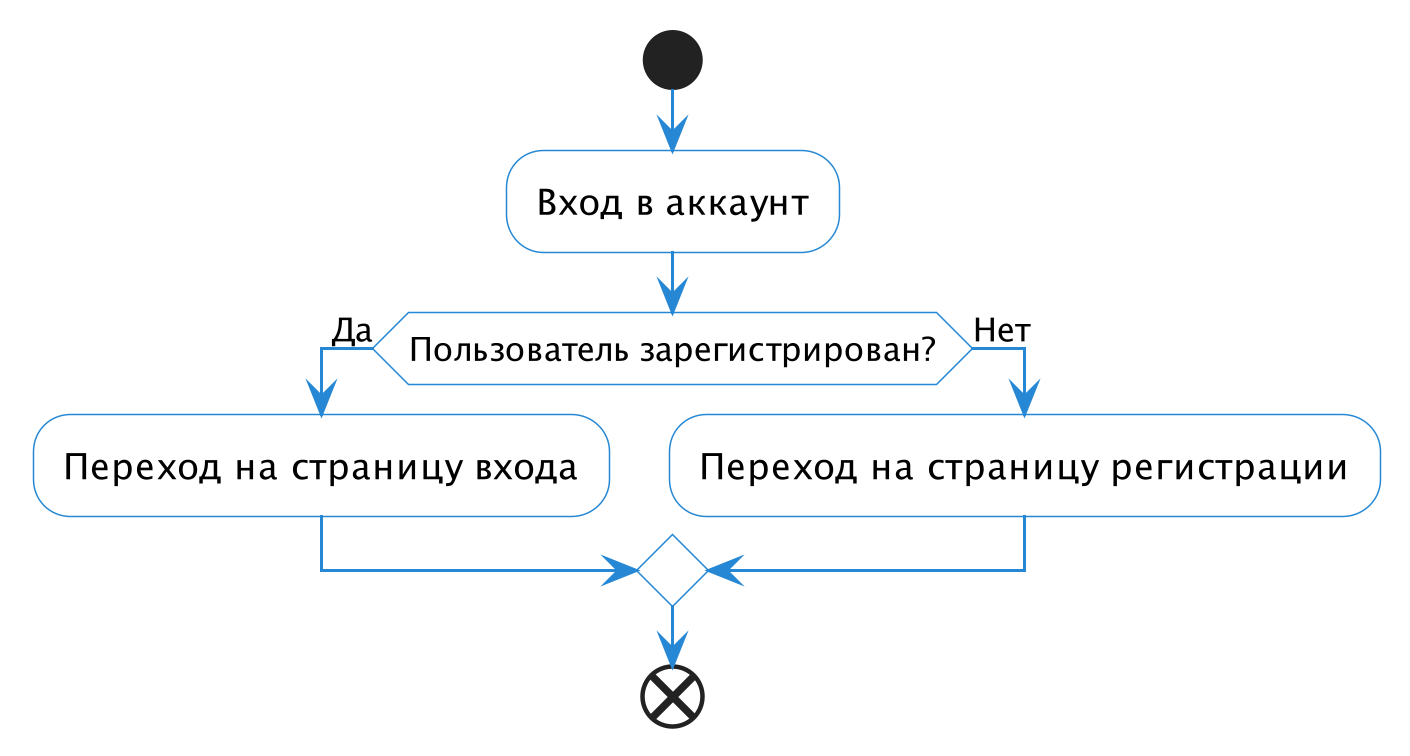
\includegraphics[width=0.95\textwidth]{images/login.png}
    \caption{Схема входа в аккаунт.}
\end{figure}

\begin{figure}[H]
    \centering
    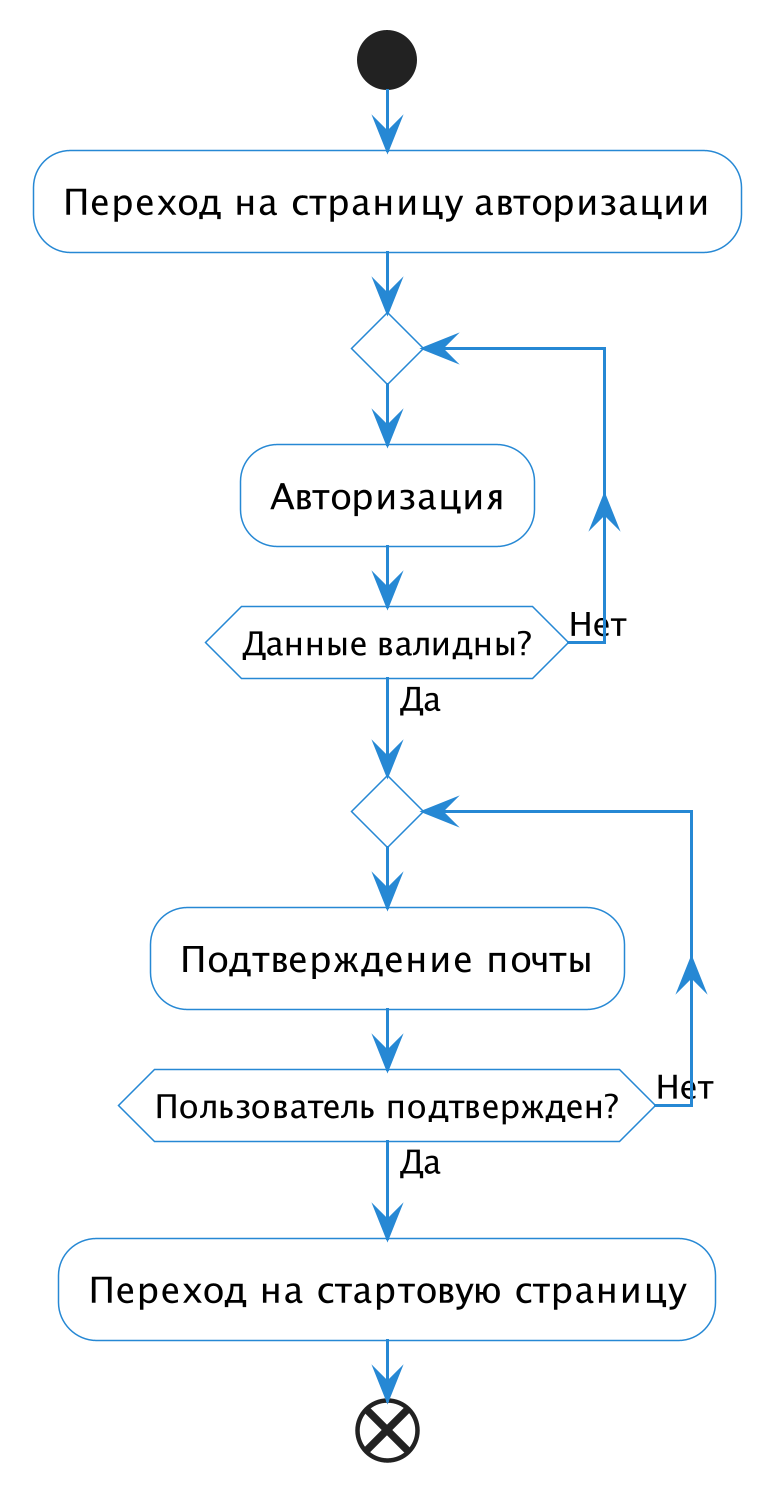
\includegraphics[height=0.65\textheight]{images/auth.png}
    \caption{Схема авторизации.}
\end{figure}

\begin{figure}[H]
    \centering
    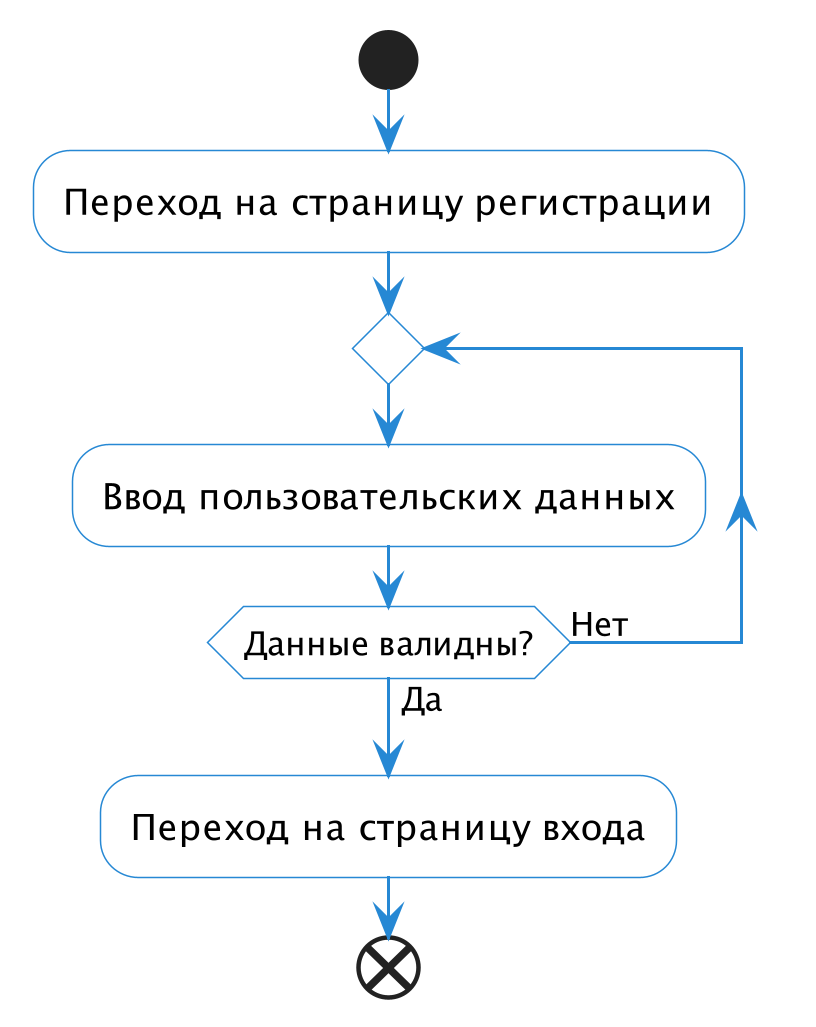
\includegraphics[height=0.5\textheight]{images/register.png}
    \caption{Схема регистрации.}
\end{figure}

\begin{figure}[H]
    \centering
    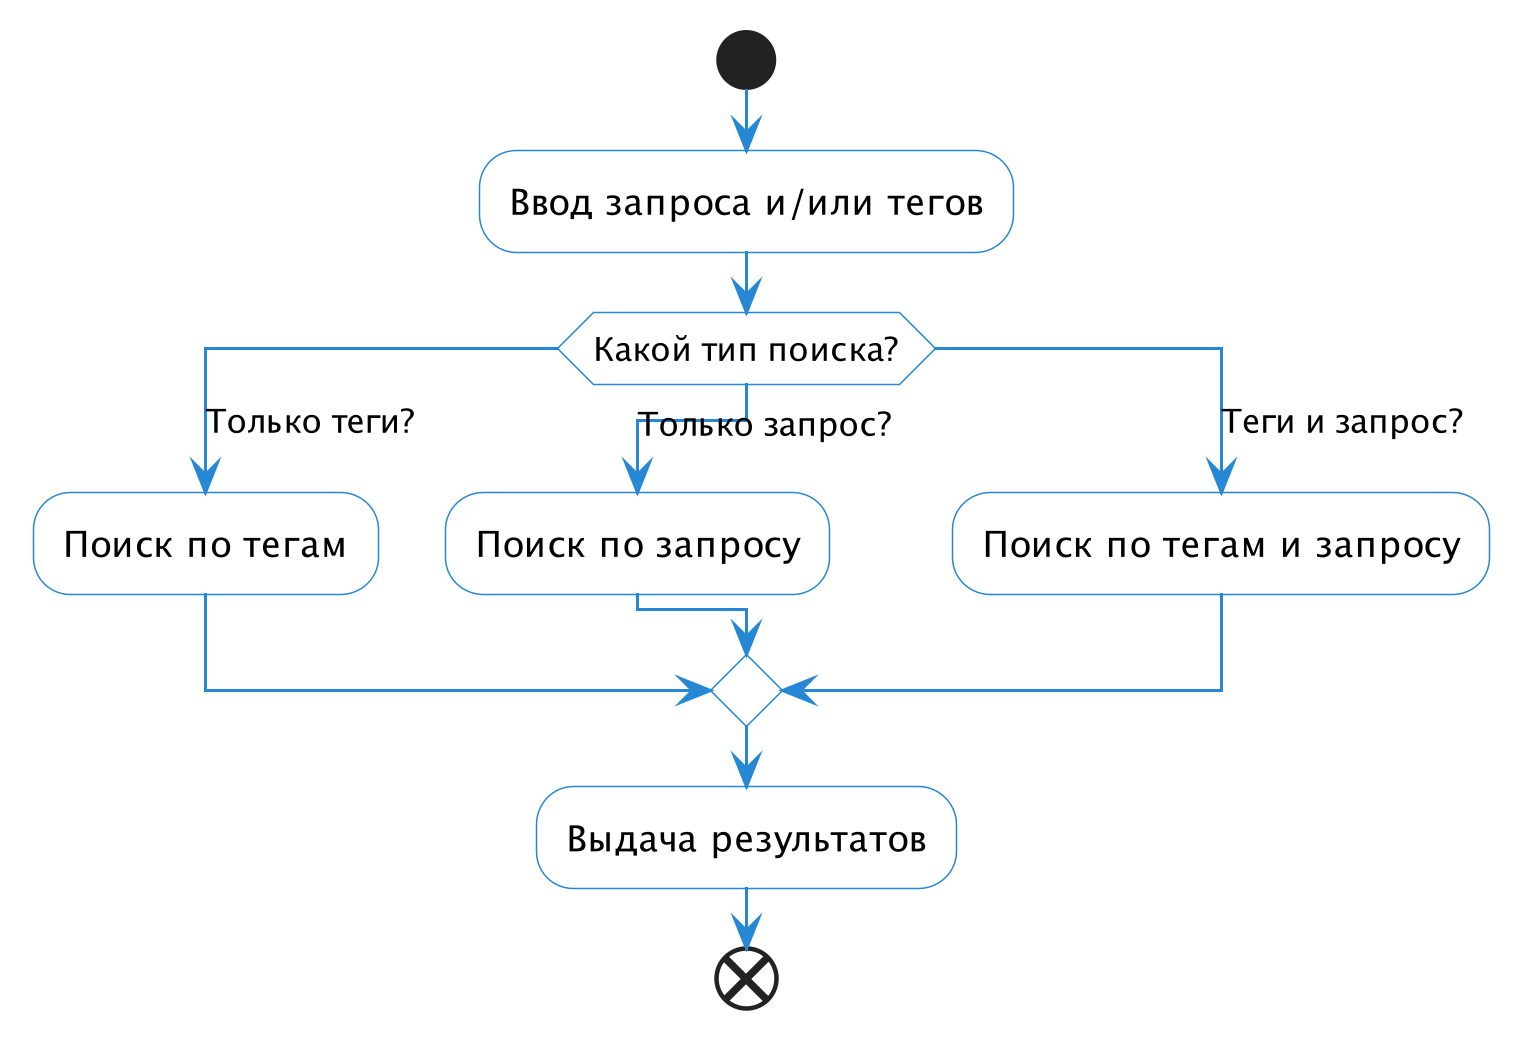
\includegraphics[width=\textwidth]{images/search.png}
    \caption{Схема поиска товаров.}
\end{figure}

\begin{figure}[H]
    \centering
    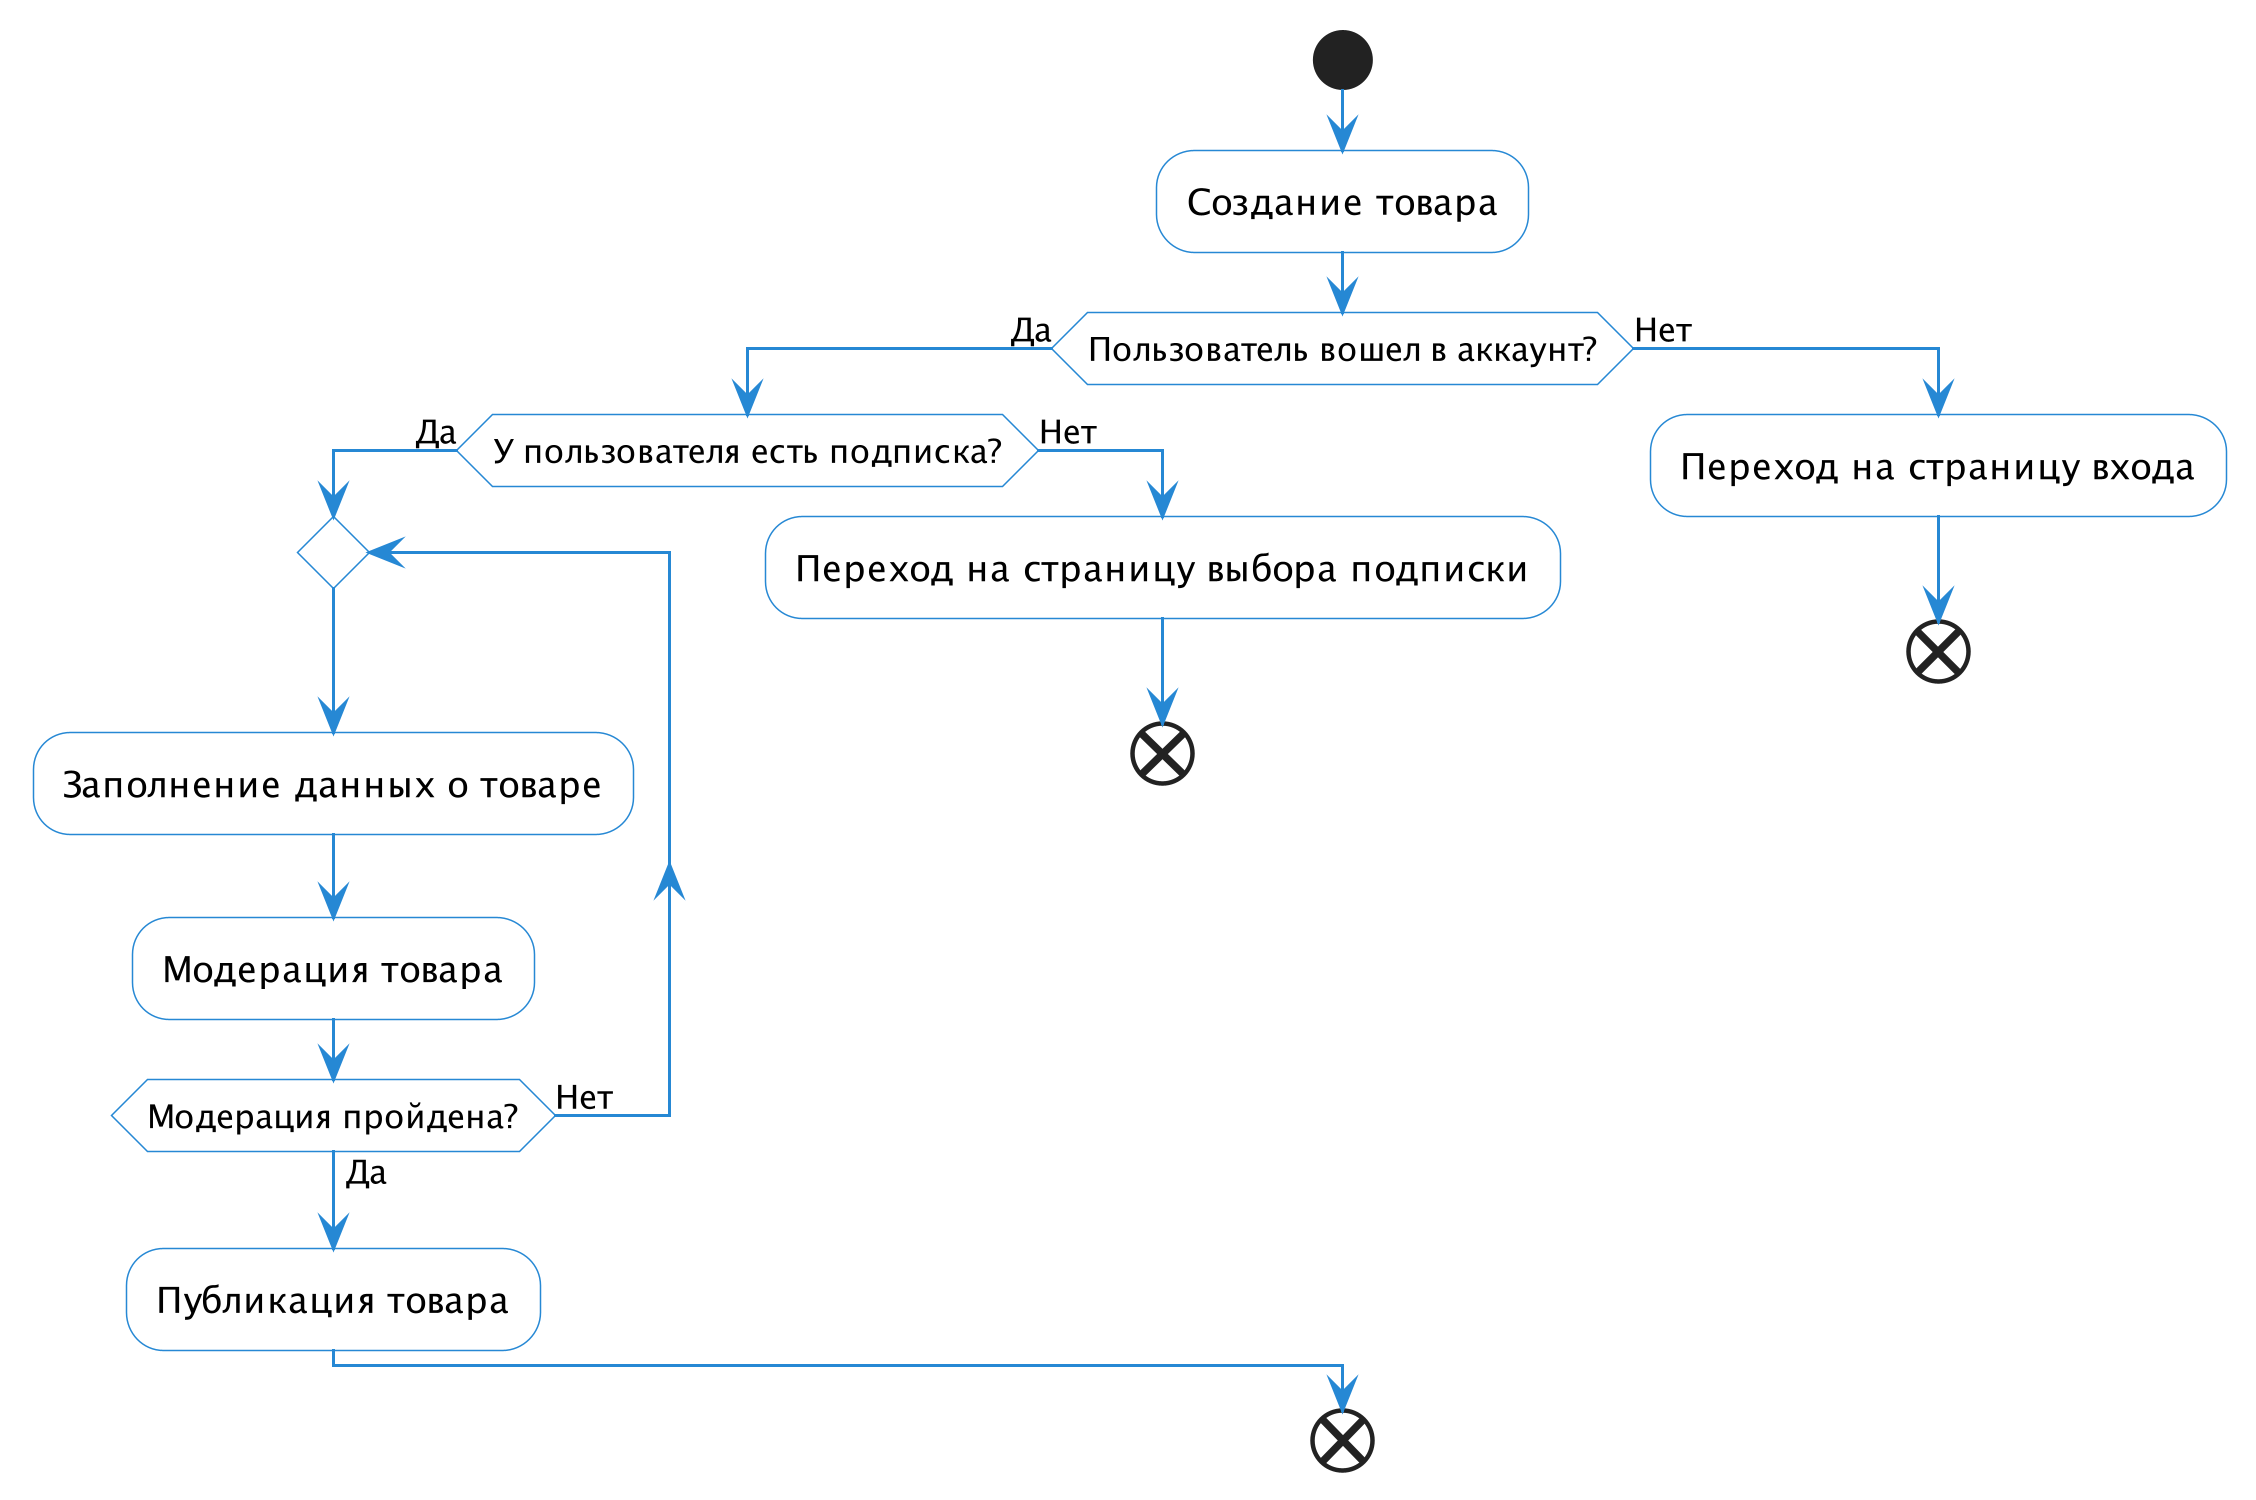
\includegraphics[width=0.95\textwidth]{images/add_item.png}
    \caption{Схема добавления товара на продажу.}
\end{figure}

\begin{figure}[H]
    \centering
    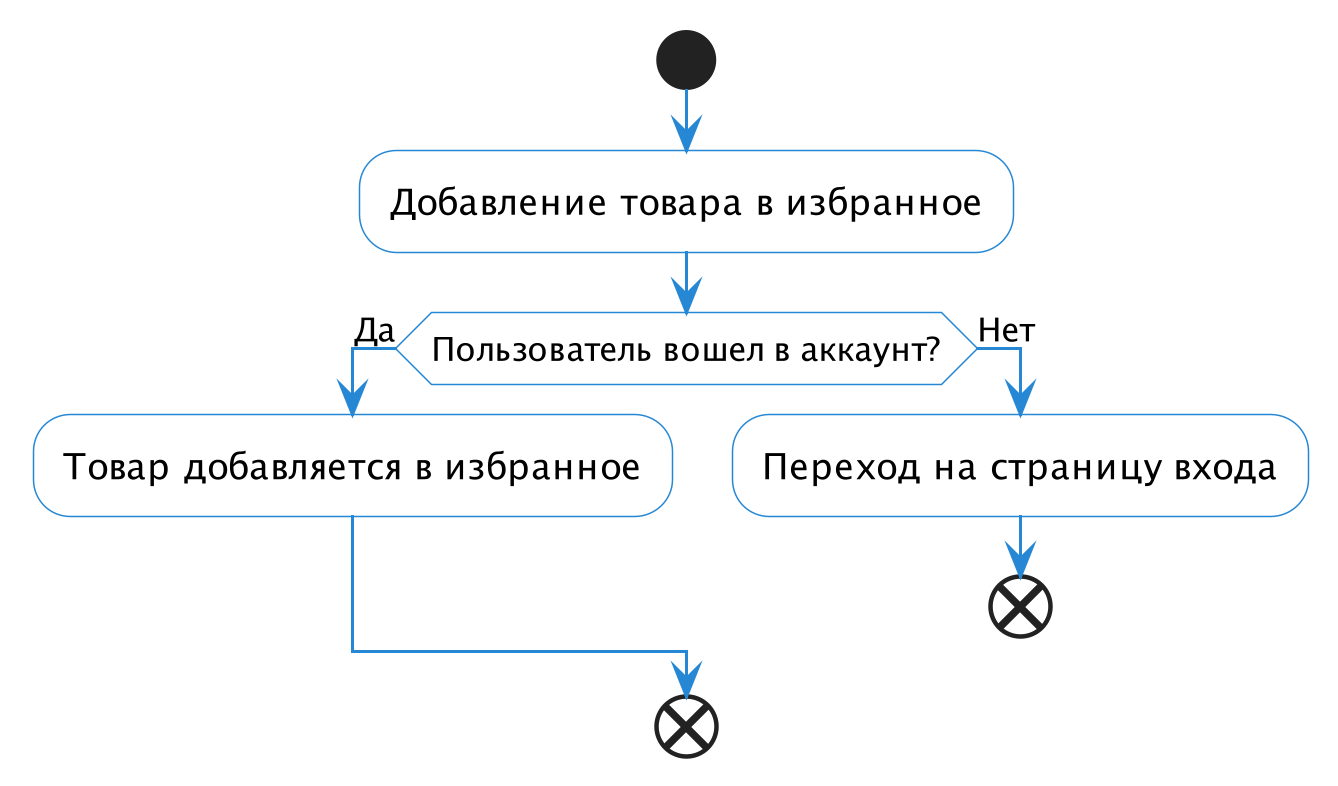
\includegraphics[width=0.95\textwidth]{images/add_to_favourites.png}
    \caption{Схема добавления товара в избранное.}
\end{figure}

\begin{figure}[H]
    \centering
    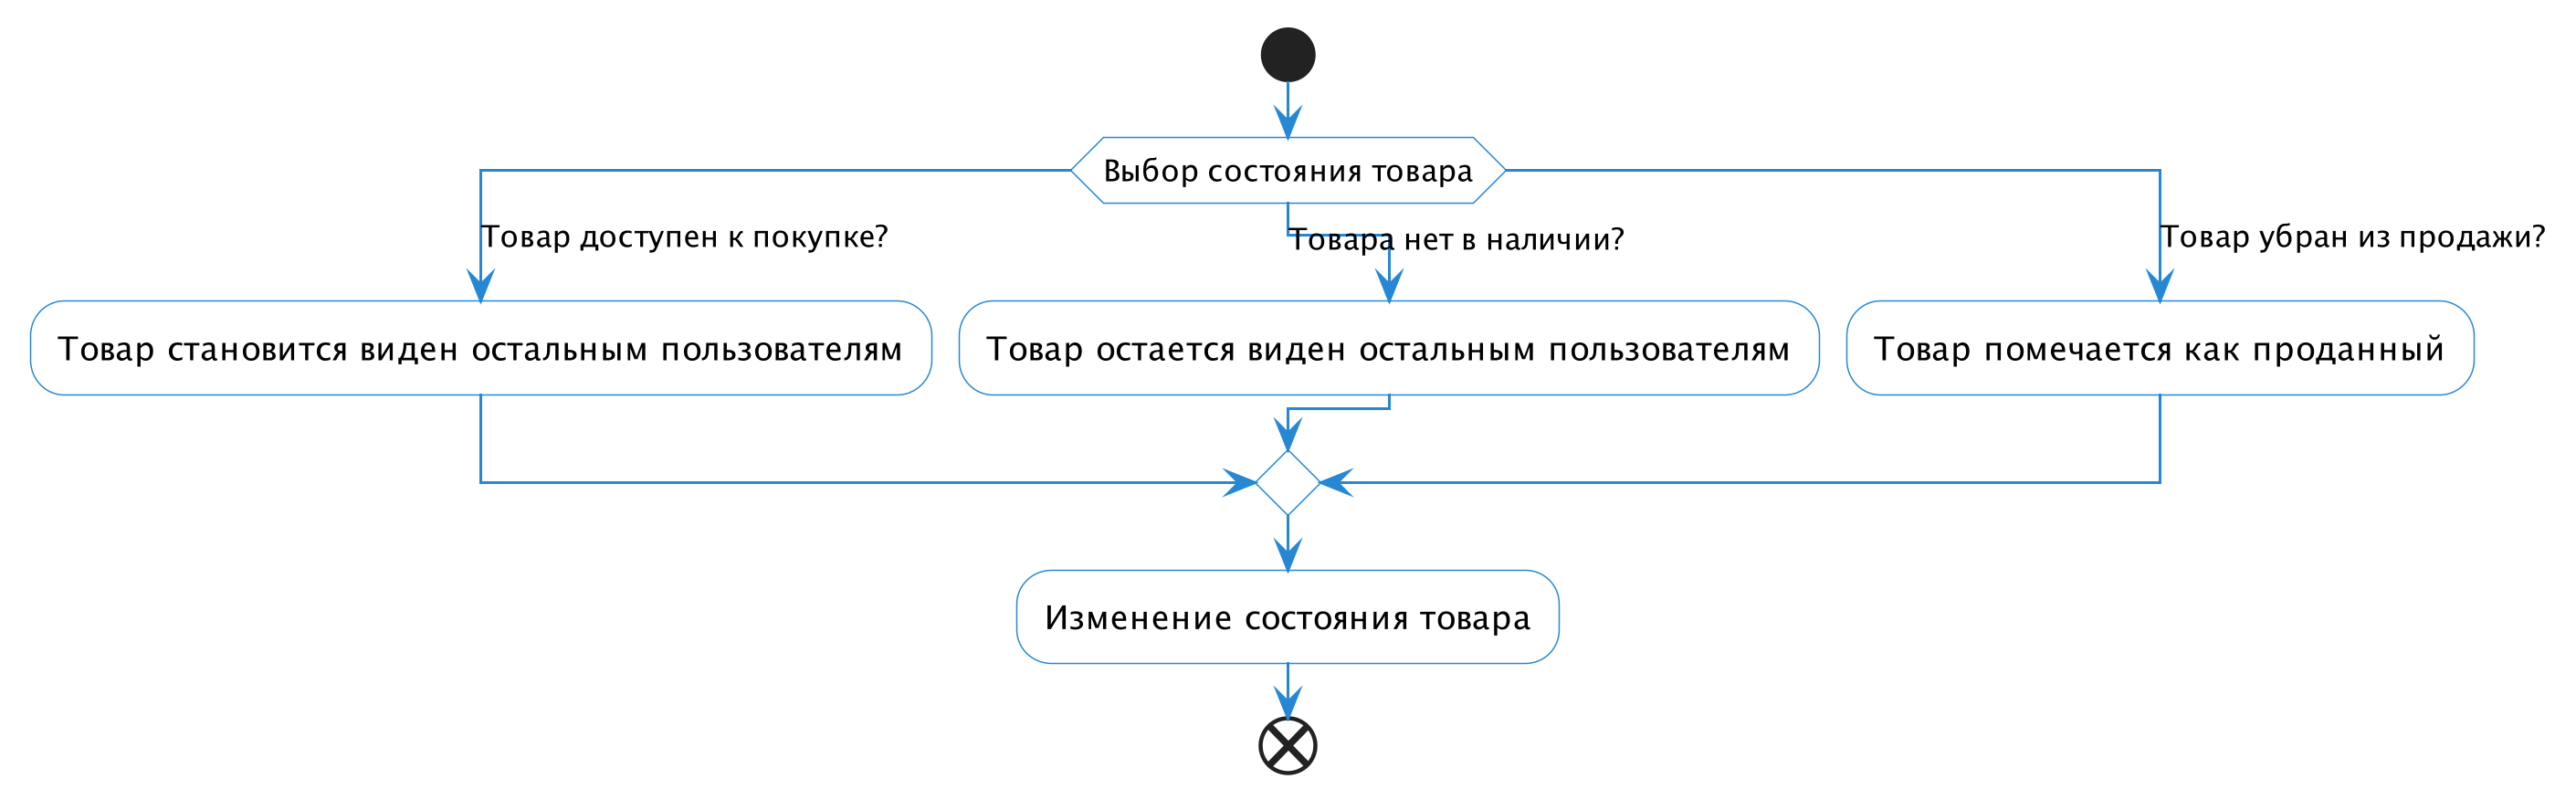
\includegraphics[width=0.95\textwidth]{images/change_item.png}
    \caption{Схема изменения состояния товара.}
\end{figure}

\begin{figure}[H]
    \centering
    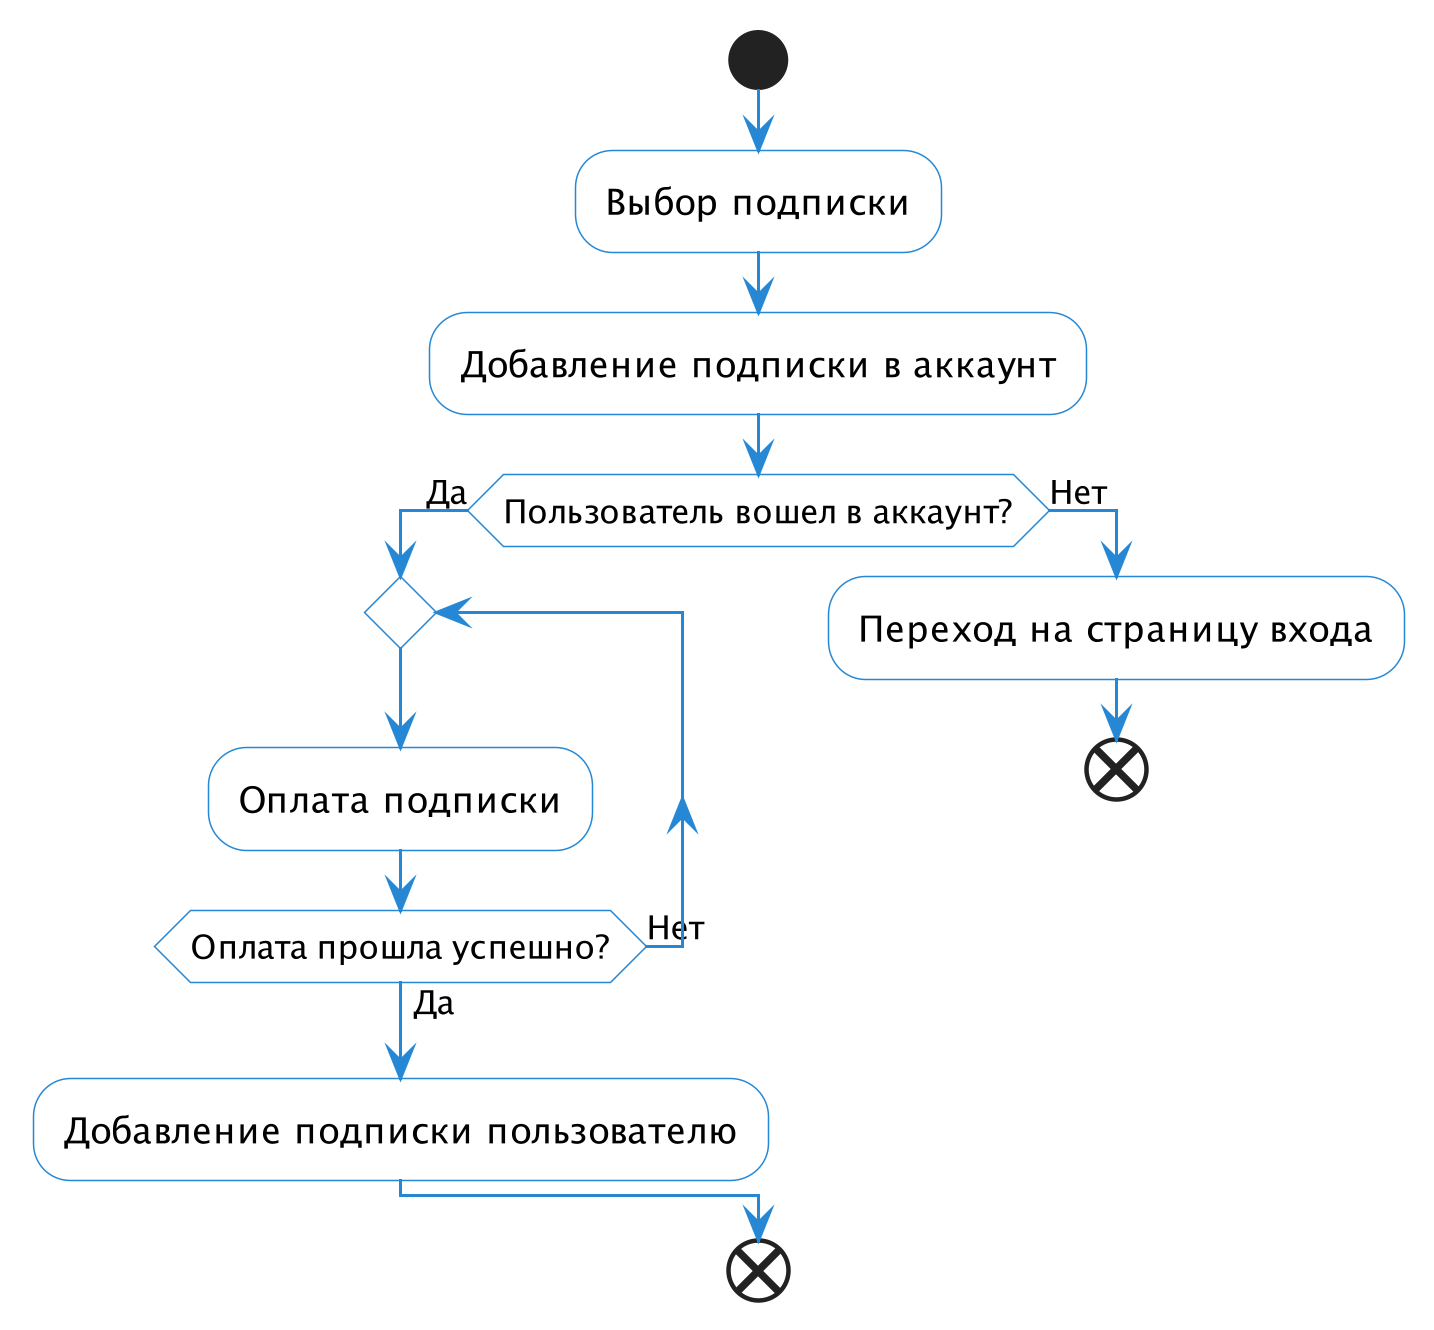
\includegraphics[width=0.95\textwidth]{images/subscription.png}
    \caption{Схема добавления подписки.}
\end{figure}

\begin{figure}[H]
    \centering
    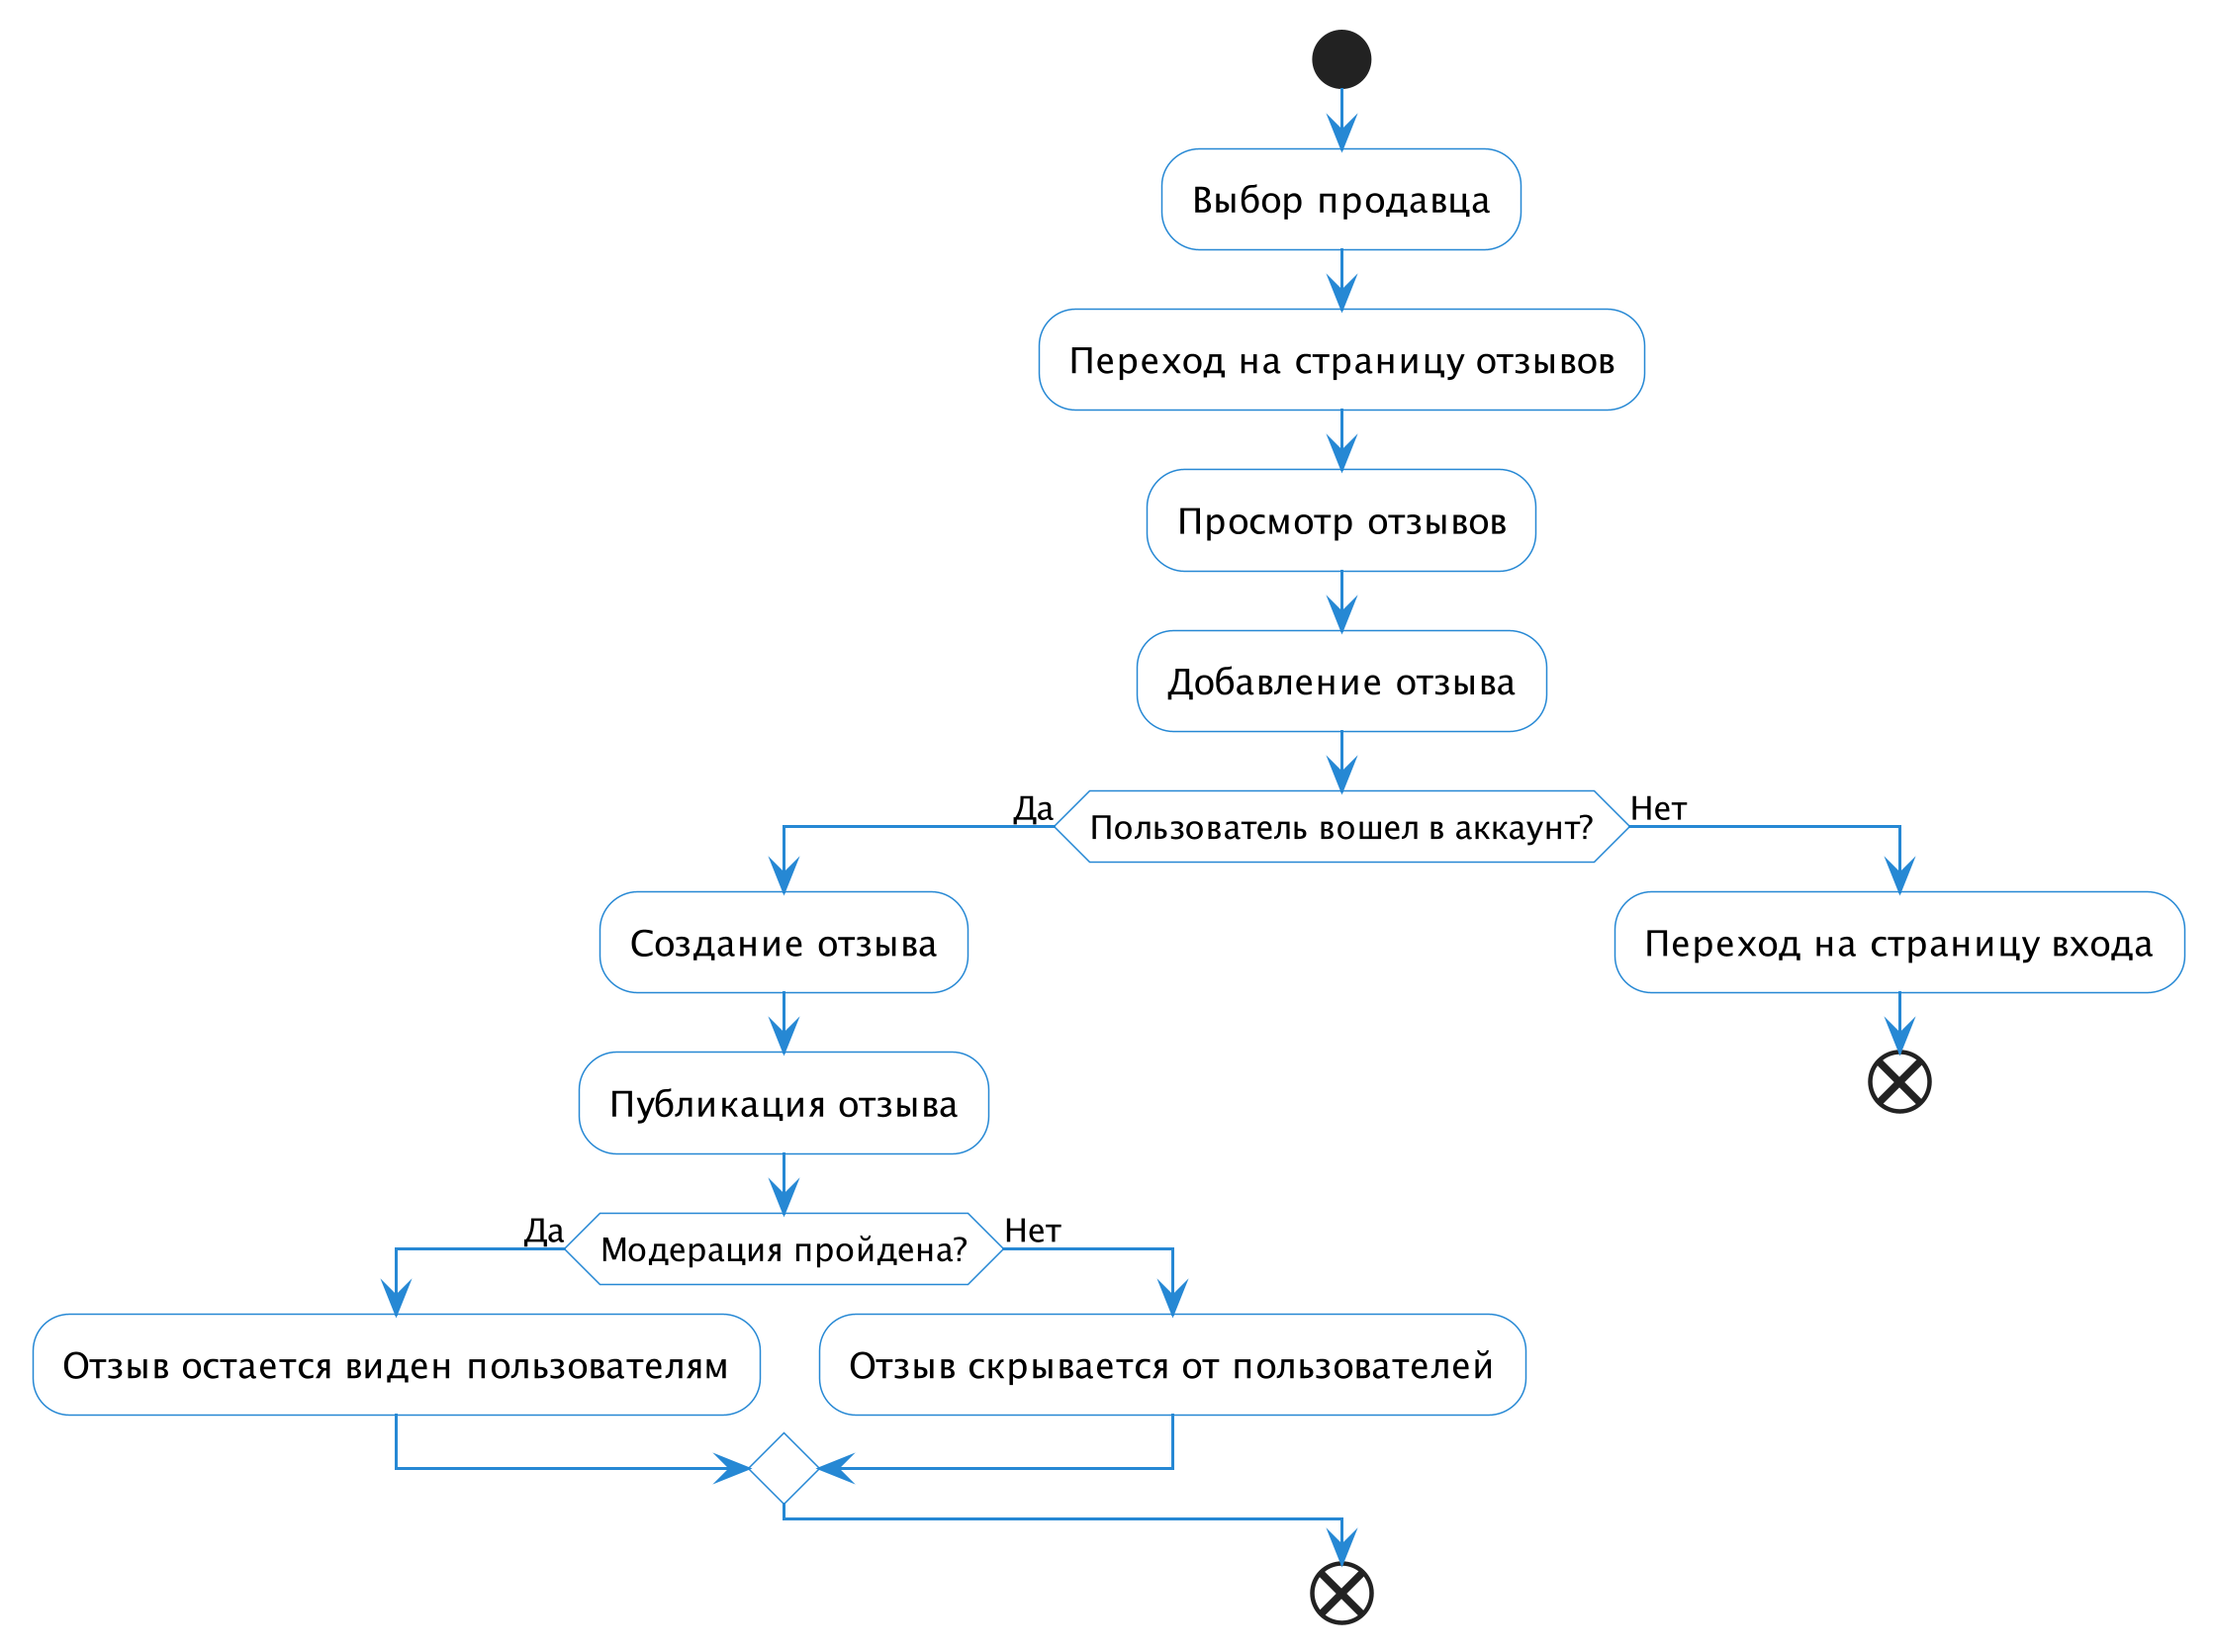
\includegraphics[width=0.95\textwidth]{images/user_feedback.png}
    \caption{Схема добавления отзыва к продавцу.}
\end{figure}

\end{document}
